
\documentclass{beamer}

\newtheorem{examplee}{Ejemplo}
\usepackage{tikz-cd}
\usepackage{svg}
\usepackage{ragged2e}
\usepackage{amsmath}
\usepackage{tikz} % Diagramas conmutativos.
\usepackage{multicol}
\mode<presentation> {
  %%% Selección de estilo
  % The Beamer class comes with a number of default slide themes
  % which change the colors and layouts of slides. Below this is a list
  % of all the themes, uncomment each in turn to see what they look like.

  %\usetheme{default}
  %\usetheme{AnnArbor}
  %\usetheme{Antibes}
  %\usetheme{Bergen}
  %\usetheme{Berkeley}
  %\usetheme{Berlin}
  %\usetheme{Boadilla}
  %\usetheme{CambridgeUS}
  %\usetheme{Copenhagen}
  %\usetheme{Darmstadt}
  %\usetheme{Dresden}
  \usetheme{Frankfurt}
  %\usetheme{Goettingen}
  %\usetheme{Hannover}
  %\usetheme{Ilmenau}
  %\usetheme{JuanLesPins}
  %\usetheme{Luebeck}
  %\usetheme{Madrid}
  %\usetheme{Malmoe}
  %\usetheme{Marburg}
  %\usetheme{Montpellier}
  %\usetheme{PaloAlto}
  %\usetheme{Pittsburgh}
  %\usetheme{Rochester}
  %\usetheme{Singapore}
  %\usetheme{Szeged}
  %\usetheme{Warsaw}

\newenvironment{ejemplo2}[3]{%
  \setbeamercolor{block body}{#2}
  \setbeamercolor{block title}{#3}
  \begin{block}{#1}}{\end{block}}
  


 \setbeamercolor{ejemplo2}{parent=structure,fg=yellow,bg=cyan}
 
  %% Selección de color
  % As well as themes, the Beamer class has a number of color themes
  % for any slide theme. Uncomment each of these in turn to see how it
  % changes the colors of your current slide theme.

  %\usecolortheme{albatross}
  %\usecolortheme{beaver}
  %\usecolortheme{beetle}
  %\usecolortheme{crane}
  %\usecolortheme{dolphin}
  %\usecolortheme{dove}
  %\usecolortheme{fly}
  %\usecolortheme{lily}
  %\usecolortheme{orchid}
  %\usecolortheme{rose}
  %\usecolortheme{seagull}
  %\usecolortheme{seahorse}
  %\usecolortheme{whale}
  %\usecolortheme{wolverine}

  %% Configuración del pie de línea
  %\setbeamertemplate{footline} % To remove the footer line in all slides uncomment this line
  %\setbeamertemplate{footline}[page number] % To replace the footer line in all slides with a simple slide count uncomment this line
  \setbeamertemplate{navigation symbols}{} % To remove the navigation symbols from the bottom of all slides uncomment this line
}
\setbeamertemplate{footline}[frame number]

%% Fuentes de tamaño arbitrario
\usepackage{lmodern}
\usepackage{graphics,tikz}
\usetikzlibrary{automata, positioning, arrows, fit, shapes}
%% Gráficos
\usepackage{graphicx} % Allows including images
\usepackage{booktabs} % Allows the use of \toprule, \midrule and \bottomrule in tables

%%% Castellano.
% noquoting: Permite uso de comillas no españolas.
% lcroman: Permite la enumeración con numerales romanos en minúscula.
% fontenc: Usa la fuente completa para que pueda copiarse correctamente del pdf.

\usepackage[spanish,es-noquoting,es-lcroman,es-tabla]{babel}
\usepackage[utf8]{inputenc}
\usepackage[T1]{fontenc}
\usepackage[linesnumbered, onelanguage]{algorithm2e}
\usepackage{tabularx}
\usepackage{listings}
\selectlanguage{spanish}
\definecolor{Maroon}{cmyk}{0, 0.87, 0.88, 0.1}
\definecolor{teal}{rgb}{0.0, 0.45, 0.45}
\newcommand{\R}{\mathbb{R}}
\newcommand{\M}{\mathcal{M}}
\newcommand{\I}{\mathcal{I}}

\renewcommand\L{\mathcal{L}}
\newcommand{\G}{\mathcal{G}}
\newcommand\m[1]{\mathcal{#1}}
%\setbeamertemplate{footline}[frame number]
%\setbeamertemplate{footline}[split theme]
%----------------------------------------------------------------------------------------
%	TÍTULO
%----------------------------------------------------------------------------------------

\title[Neurociencia computacional]{Herramientas y estrategias de parameter tuning aplicadas a la neurociencia computacional} % The short title appears at the bottom of every slide, the full title is only on the title page

\author{Andrés Arco López} % Your name
\institute[UGR] % Your institution as it will appear on the bottom of every slide, may be shorthand to save space
{
  Universidad de Granada \\ % Your institution for the title page
  \medskip
  \textit{Grado en Ingeniería Informática} % Your email address
}

\date{22 de Noviembre de $2022$} % Date, can be changed to a custom date


\AtBeginSection[]{
	\begin{frame}
		\vfill
		\centering
		\begin{beamercolorbox}[sep=8pt,center,shadow=true,rounded=true]{title}
			\usebeamerfont{title}\insertsectionhead\par%
		\end{beamercolorbox}
		\vfill
	\end{frame}
}


\begin{document}

%% Diapositiva de título.
\frame[plain]{
\titlepage % Print the title page as the first slide
\small{\textit{Trabajo tutorizado por Pablo Martínez Cañada}}
}

%% Diapositiva de contenidos.
% Throughout your presentation, if you choose to use \section{} and \subsection{} commands, 
% these will automatically be printed on this slide as an overview of your presentation

\frame[plain]{
  \frametitle{Contenidos} % Table of contents slide, comment this block out to remove it
  \tableofcontents
}


%----------------------------------------------------------------------------------------
%	PRESENTACIÓN
%----------------------------------------------------------------------------------------

%------------------------------------------------
\section{Motivación de este TFG} 


\begin{frame}{¿Por qué usar modelos de simulación del cerebro?}

Actualmente, conocemos menos del 10\% del funcionamiento del cerebro. La neurociencia computacional permite construir modelos de simulación del cerebro, que incluyen cientos de miles de neuronas para:

\vfill
\pause
\setbeamertemplate{items}[triangle]
\begin{itemize}
    \item \textbf{Diseñar algoritmos} que descubren cómo resolver problemas neurológicos.
    \vspace{2mm}
    \pause
    \item \textbf{Crear nuevas herramientas} para el diagnóstico de enfermedades.
    \vspace{2mm}
    \pause
    \item Explorar \textbf{hipótesis sobre la función del cerebro} que la neurociencia experimental no es capaz con los métodos existentes de registro neuronal.
    \vspace{2mm}  
\end{itemize}

\vspace{5mm}

\end{frame}

\begin{frame}{Objetivos principales}

Conseguir \textbf{estimar los parámetros del modelo} (por ejemplo, el cociente entre excitación, E, e inhibición, I: E/I) que han dado lugar a las distintas propiedades de la señal del EEG.

\vspace{4mm}
\pause

 Desarrollar \textbf{herramientas} que podrían ser usadas para ayudar en el \textbf{diagnóstico clínico de condiciones médicas} y descodificar los parámetros del circuito cortical que son alterados.

\end{frame}

\section{Métodos}
 
\begin{frame}{Modelo neuronal}

Para poder llevar a cabo todas las simulaciones se ha usado NEST, que es un simulador de red neuronal de spikes utilizado para simular dinámicas de interacción entre neuronas. 

\vfill
\pause
\setbeamertemplate{items}[triangle]
    \begin{itemize}
        \item El modelo cuenta con un total de 5000 neuronas, de las cuales, 4000 excitatorias y 1000 inhibitorias.
        \vspace{2mm}
        \pause
        \item Se estudia el comportamiento de estas neuronas en intervalos de 1 ms (1000 puntos de actividad neuronal en cada simulación).
        \vspace{2mm}
        \pause
        \item Se han obtenido resultados a partir de la variación de 5 parámetros.
        \vspace{2mm}  
    \end{itemize}    

\end{frame}


\begin{frame}{Modelo neuronal}
\begin{figure}
      \centering
      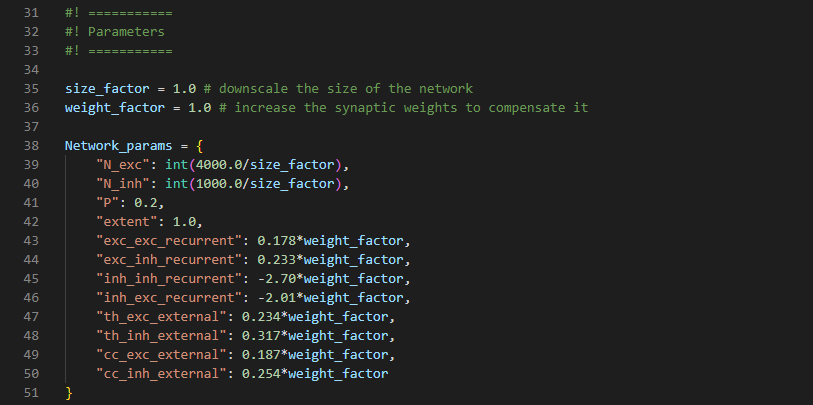
\includegraphics[scale=0.6]{memoria/images/Código parámetros.png}
      \caption{Código donde se representan los valores de referencia de las conductancias sinápticas.}
\end{figure}
\end{frame}

\begin{frame}{Paralelización en el servidor}

La paralelización puede mejorar la eficiencia de la ejecución de simulaciones a gran
escala aprovechando máquinas multinúcleo/multiprocesador, clústeres de computadoras
o supercomputadoras. Para la realización de las simulaciones se ha utilizado:

\vfill
\pause
\setbeamertemplate{items}[triangle]
    \begin{itemize}
        \item Un servidor con sistema operativo Linux que cuenta con 32 núcleos disponibles.
        \vspace{2mm}
        \pause
        \item Memoria RAM de 128GB y almacenamiento de hasta 2TB de información.
        \vspace{2mm}
        \pause
        \item Se han realizado un total de 480 simulaciones (4 minutos por simulación).
        \vspace{2mm}  
        \pause
        \item Conjunto de datos compuesto por archivos: .spikes, .AMPA, .GABA.
        \vspace{2mm} 
    \end{itemize}    

\end{frame}

\begin{frame}{Análisis de los datos}

Para el cálculo de la señal del electroencefalograma EEG, se ha hecho uso de la siguiente fórmla, que en trabajos previos ha demostrado aproximar bien el EEG (Martínez-Cañada et al. [2021]).

   $$ EEG = |AMPA| + |GABA| $$
\pause
Ahora se mostrarán los distintos tipos de gráficas obtenidas al variar los parámetros de las simulaciones.

\end{frame}


\begin{frame}{Análisis de los datos}
\begin{figure}
\centering
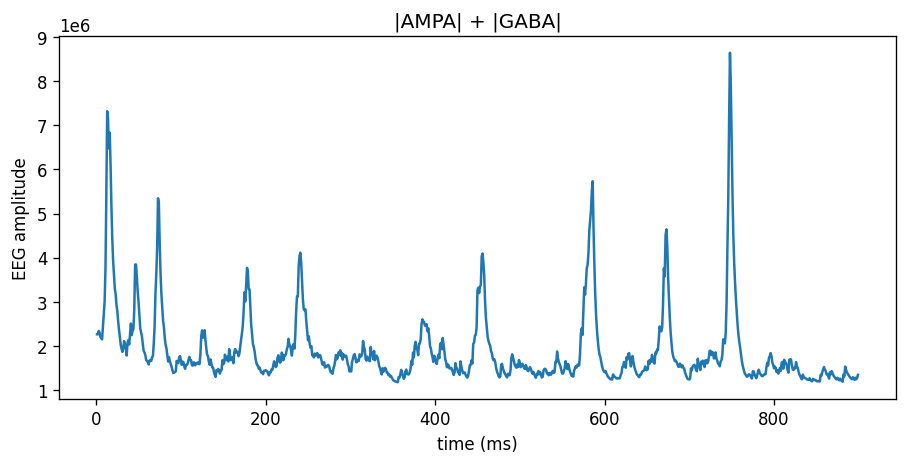
\includegraphics[width=10cm]{memoria/images/EEG-Estandar.png}
\caption{Gráfica del EEG con valores estándar}
\end{figure}


\end{frame}

\begin{frame}{Análisis de los datos}

\begin{figure}
    \centering
    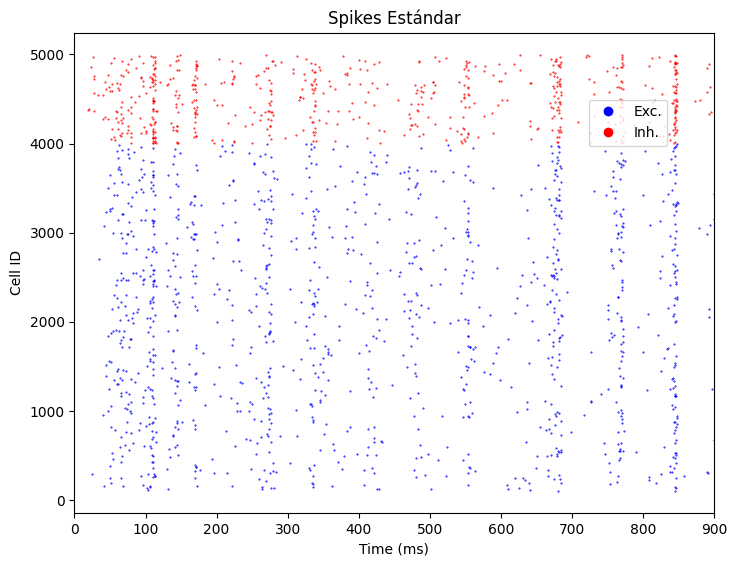
\includegraphics[width=9cm]{memoria/images/Spikes-Estandar.png}
    \caption{Gráfica de spikes con valores estándar}
\end{figure}


\end{frame}

\begin{frame}{Análisis de los datos}
\begin{figure}
\centering
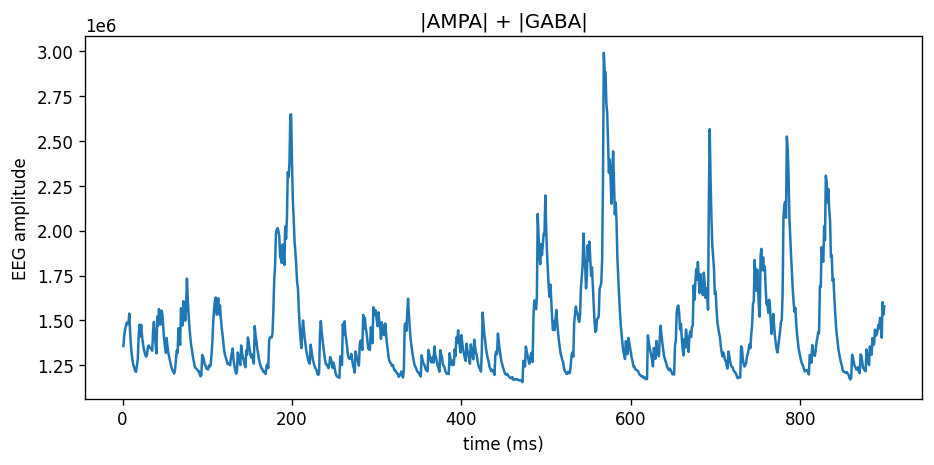
\includegraphics[width=10cm]{memoria/images/EEG-Exc_Exc-0.005.png}
\caption{Gráfica del EEG con parámetro exc\_exc = -0.005.}
\end{figure}


\end{frame}

\begin{frame}{Análisis de los datos}

\begin{figure}
    \centering
    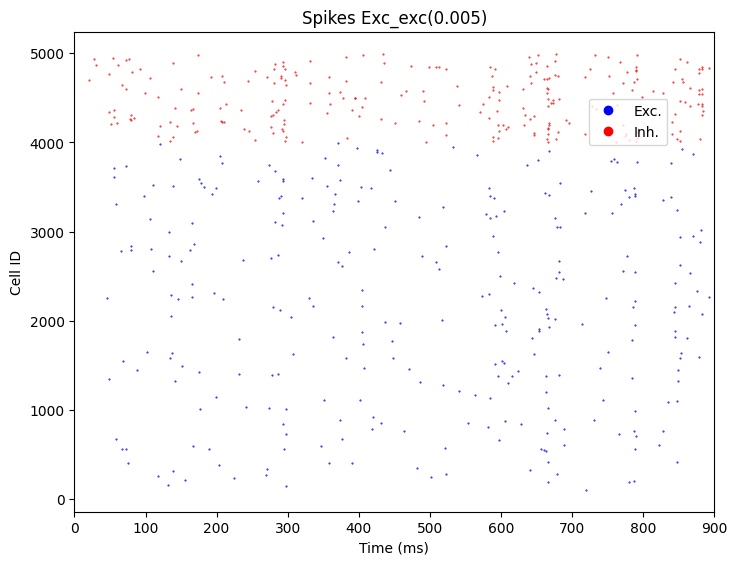
\includegraphics[width=9cm]{memoria/images/Spikes-Exc_Exc-0.005.png}
    \caption{Gráfica de spikes con parámetro exc\_exc = -0.005.}
\end{figure}


\end{frame}

\begin{frame}{Conjunto de datos del estudio}

Estos valores del EEG se han almacenado en una variable $X$ en la que en la que en cada elemento tenemos un vector con todos los valores del EGG de esa simulación y otra variable $Y$ multidimensional que se corresponden con los valores de los ratios de conductancias $g$ calculados como:


 $$   g = \frac{g\_exc}{g\_inh} $$


y con con los valores de la entrada externa del modelo (que puede representar la entrada del tálamo) $v_0$.


\end{frame}

\begin{frame}{Algoritmos de Machine Learning}

Los algoritmos que se han utilizado para estimar los parámetros del modelo, g y $v_0$, han sido:

\vfill
\pause
\setbeamertemplate{items}[triangle]
    \begin{itemize}
        \item Algoritmo de regresión lineal simple.
        \vspace{2mm}
        \pause
        \item Algoritmo de regresión de Ridge (variando el parámetro alfa).
        \vspace{2mm}
        \pause
        \item Algoritmo no lineal - K-Nearest Neighbors.
        \vspace{2mm}  
        \pause
        \item Algoritmo no lineal - Red Neuronal.
        \vspace{2mm} 
    \end{itemize}  
 \pause

\end{frame}

\begin{frame}{Algoritmos de Machine Learning}

Se ha hecho uso de la librería scikit-learn en Python, para la ejecución de todos ellos excepto para la Red Neuronal, que ha requerido la utilización de una función externa usada en otros estudios.

Para el estudio de los resultados obtenidos con cada algoritmo se han realizado 100 repeticiones de 10-fold cross validation, en las cuales, se seleccionan aleatoriamente los datos de entrenamiento y los datos de test.

\end{frame}

\section{Resultados}
 
\begin{frame}{Regresión lineal simple}
    
\begin{figure}
\centering
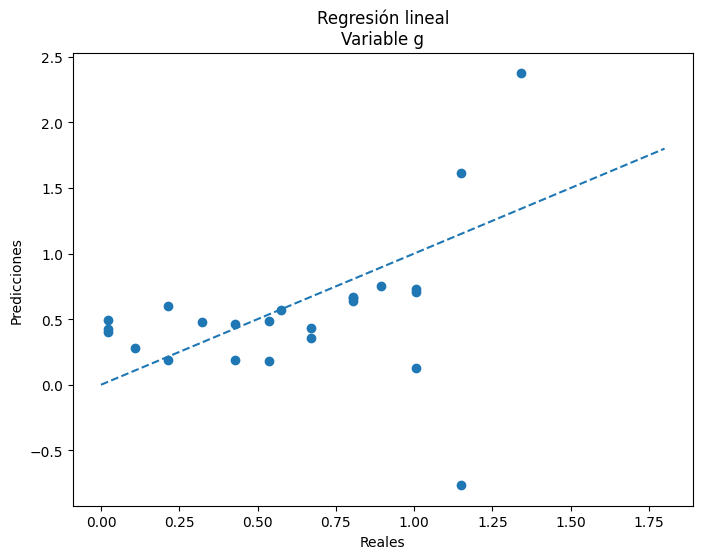
\includegraphics[width=7cm]{memoria/images/Regresión lineal Variable g.png}
\caption{Comparativa entre los valores reales y las predicciones de la variable g para 1 fold de 10-fold cross validation.}
\end{figure}

\end{frame}

\begin{frame}{Regresión lineal simple aplicando autocorrelación}
    
\begin{figure}
\centering
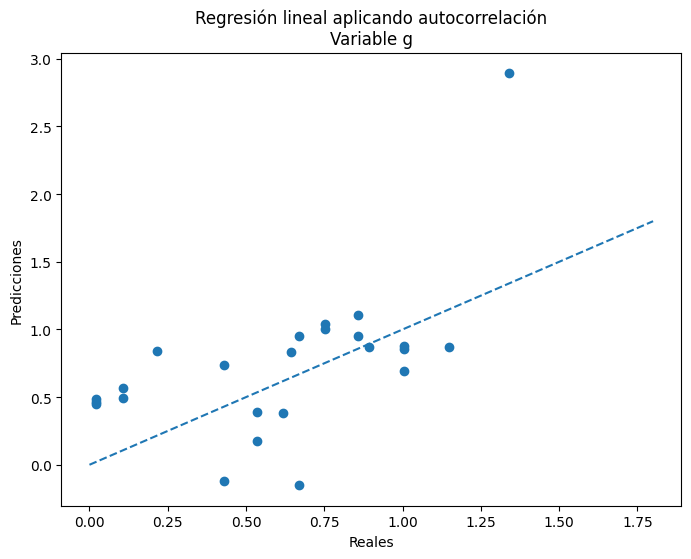
\includegraphics[width=7cm]{memoria/images/Regresión lineal aplicando autocorrelación Variable g.png}
\caption{Comparativa entre los valores reales y las predicciones de la variable g después de aplicar autocorrelación para 1 fold de 10-fold cross validation.}
\end{figure}

\end{frame}

\begin{frame}{Regresión de Ridge (alfa = 0.5)}
    
\begin{figure}
\centering
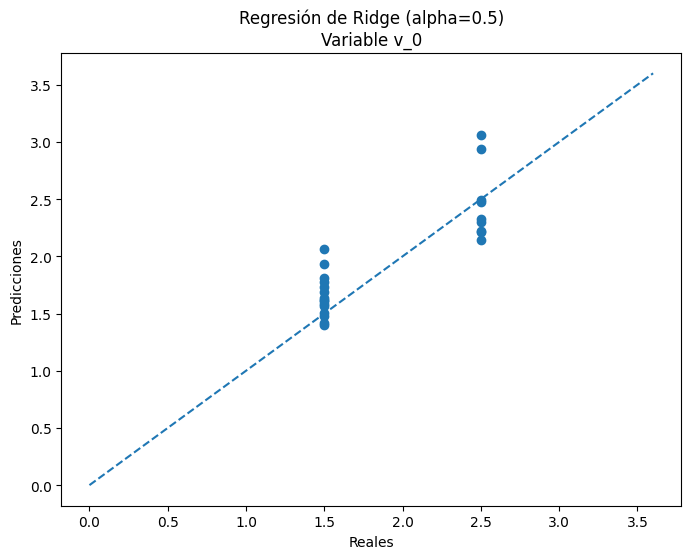
\includegraphics[width=7cm]{memoria/images/Regresión de Ridge (alpha=0.5) Variable v_0.png}
\caption{Comparativa entre los valores reales y las predicciones de la variable $v_0$ para 1 fold de 10-fold cross validation.}
\end{figure}

\end{frame}

\begin{frame}{Regresión de Ridge aplicando autocorrelación (alfa = 0.5)}
    
\begin{figure}
\centering
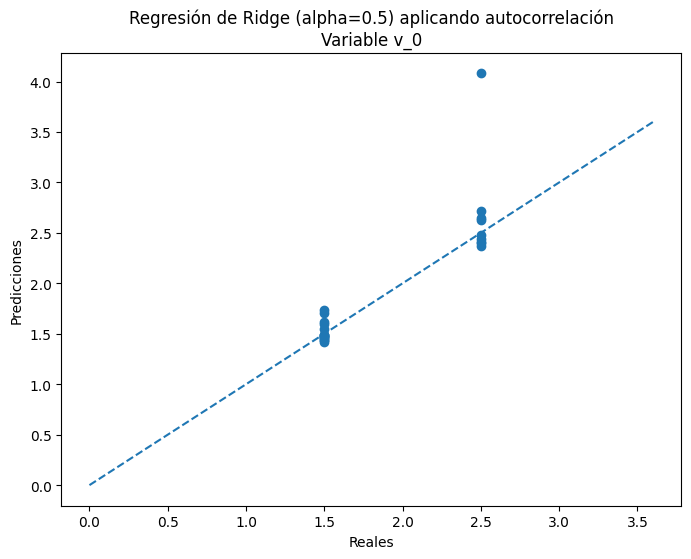
\includegraphics[width=7cm]{memoria/images/Regresión de Ridge (alpha=0.5) aplicando autocorrelación Variable v_0.png}
\caption{Comparativa entre los valores reales y las predicciones de la variable $v_0$ después de aplicar autocorrelación para 1 fold de 10-fold cross validation.}
\end{figure}

\end{frame}

\begin{frame}{K-Nearest Neighbors}
    
\begin{figure}
\centering
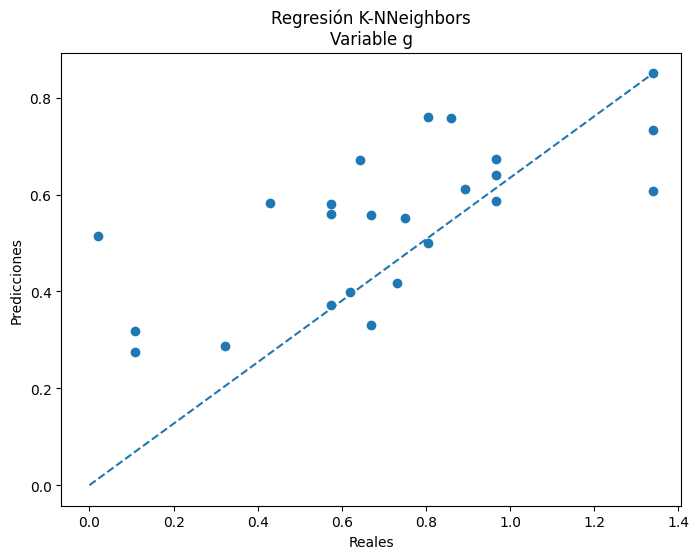
\includegraphics[width=7cm]{memoria/images/Regresión K-NNeighbors Variable g.png}
\caption{Comparativa entre los valores reales y las predicciones de la variable g para 1 fold de 10-fold cross validation.}
\end{figure}

\end{frame}

\begin{frame}{K-Nearest Neighbors aplicando autocorrelación}
    
\begin{figure}
\centering
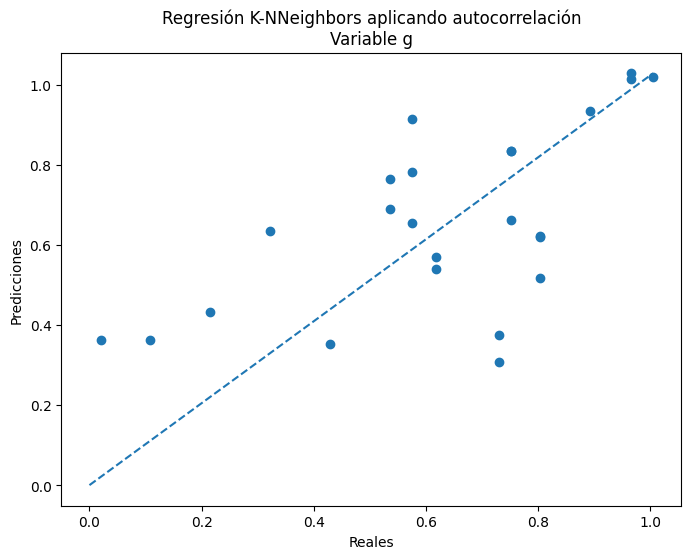
\includegraphics[width=7cm]{memoria/images/Regresión K-NNeighbors aplicando autocorrelación Variable g.png}
\caption{Comparativa entre los valores reales y las predicciones de la variable g después de aplicar autocorrelación para 1 fold de 10-fold cross validation.}
\end{figure}

\end{frame}

\begin{frame}{Resultados finales}
    
Tras realizar un total de 1000 ejecuciones mediante cada uno de los algoritmos (excepto en el de Red Neuronal, debido a su complejidad) y almacenar promedio de todos los errores cuadráticos medios calculados en cada ejecución, entre los valores de test y los valores obtenidos en las predicciones, se han obtenido los siguientes resultados.

\end{frame}

\begin{frame}{Todos los resultados}
    
\begin{figure}
\centering
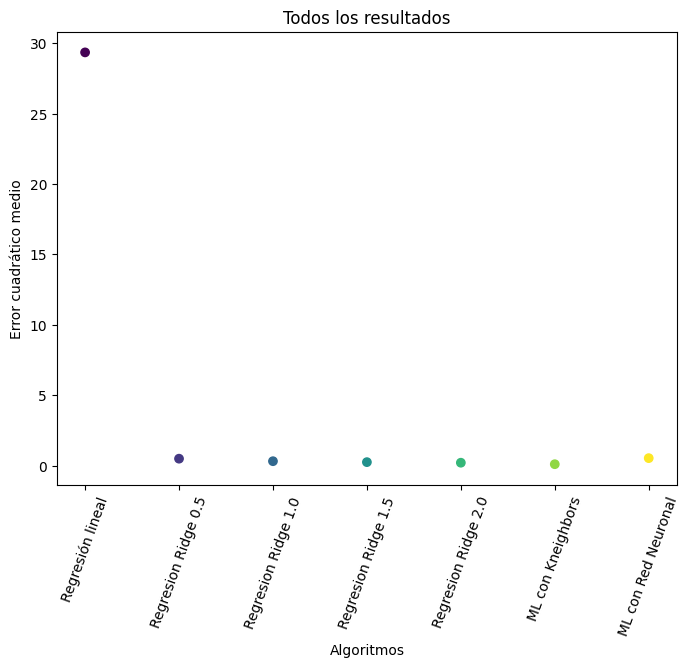
\includegraphics[width=8cm]{memoria/images/Todos los resultados.png}
\end{figure}

\end{frame}

\begin{frame}{Todos los resultados con autocorrelación}
    
\begin{figure}
\centering
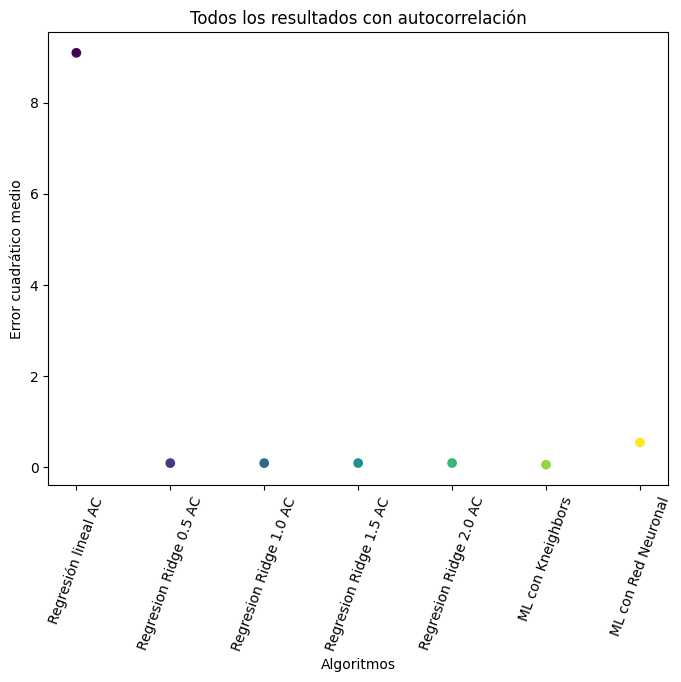
\includegraphics[width=8cm]{memoria/images/Todos los resultados con autocorrelación.png}
\end{figure}

\end{frame}

\begin{frame}{Mejores resultados}
    
\begin{figure}
\centering
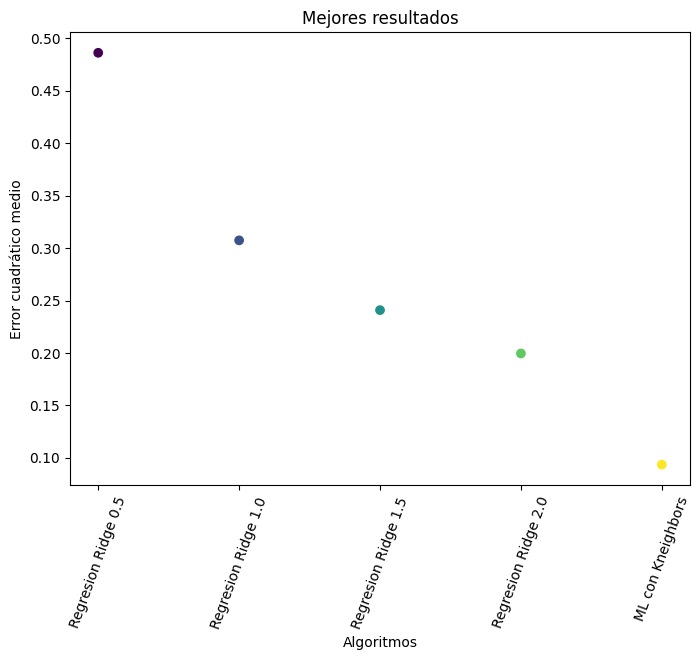
\includegraphics[width=8cm]{memoria/images/Mejores resultados.png}
\end{figure}

\end{frame}

\begin{frame}{Mejores resultados con autocorrelación}
    
\begin{figure}
\centering
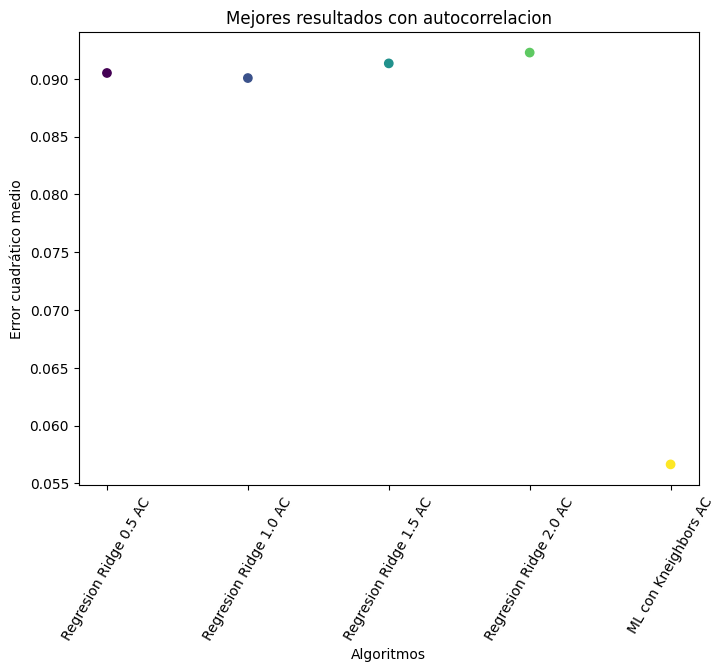
\includegraphics[width=8cm]{memoria/images/Mejores resultados con autocorrelación.png}
\end{figure}

\end{frame}

\section{Conclusiones y vías futuras}

\begin{frame}{Conclusiones}

    \begin{itemize}
    \justifying
      \item Hemos obtenido un gran conjunto de datos, entre ellos la señal del electroencefalograma (EEG), que es una de las señales no-invasivas más conocida en el ámbito clínico.
      \vspace{2mm}
      \pause
      \item Analizando estas señales hemos sido capaces de detectar diferentes tipos de gráficas, algunas muy realistas.
      \vspace{2mm}
      \pause
      \item Hemos estimado variaciones del parámetro E/I, que según la literatura están relacionadas con patologías como la epilepsia o el autismo.
      \vspace{2mm}
      \pause
      \item Gracias a estos algoritmos y usando un modelo del cerebro, hemos podido leer señales del EEG y producir estimaciones de cambios en E/I, obteniendo los mejores resultados con el algoritmo de K-Nearest Neighbors.
    \end{itemize}
\end{frame}

\begin{frame}{Limitaciones}

\begin{itemize}
    \justifying
    \item El modelo cerebral usado es un modelo simplificado de una pequeña parte del cerebro y no tiene en cuenta conexiones con otras regiones del cerebro.
    \vspace{4mm}    
    \pause
    \item El modelo usa neuronas de tipo de LIF, que son neuronas simplificadas, que facilitan el cálculo del potencial con vistas a su implementación hardware
    \vspace{4mm}
    \pause
    \item La fórmula utilizada para generar el EEG, es una fórmula simplificada, con la que hemos sido capaces de mantenernos cercanos a los valores esperados, pero no tienen en cuenta otros factores.
    
\end{itemize}
\end{frame}


\begin{frame}{Trabajo futuro}

\begin{itemize}
    \justifying
    \item Mejorar el modelo superando las limitaciones mencionadas anteriormente, haciendo uso de una mayor cantidad de parámetros.
    \vspace{4mm}    
    \pause
    \item Aplicar el modelo a registros reales de señales del EEG tomados en pacientes con patologías clínicas.
    
\end{itemize}
\end{frame}




%% Bibliografía
\begin{frame}{Bibliografía fundamental}
\begin{itemize}
  \item Noei S. Martínez-Cañada, P. and S. Panzeri. Methods for inferring neural circuit interactions and neuromodulation from local field potential and electroencephalogram measures. Brain Informatics, 8, 2021. 
  \item Pablo Martínez-Cañada, Torbjørn V. Ness, Gaute T. Einevoll, Tommaso Fellin, and Stefano Panzeri. Computation of the electroencephalogram (eeg) from network models of point neurons. PLOS Computational Biology, 17:1–41, 04 2021.
  \item Alberto Mazzoni, Stefano Panzeri, Nikos K. Logothetis, and Nicolas Brunel. Encoding of naturalistic stimuli by local field potential spectra in networks of excitatory and inhibitory neurons. PLOS Computational Biology, 4, 12 2008. 
 
\end{itemize}

\end{frame}


\begin{frame}{Bibliografía fundamental}
\begin{itemize}
    \item Whittingstall K. Brunel N. Logothetis N. K. Panzeri S. Mazzoni, A. Understanding the relationships between spike rate and delta/gamma frequency bands of lfps and eegs using a local cortical network model. page 956–972, 2010.
    \item Merzenich M. M. Rubenstein, J. L. Model of autism: increased ratio of excitation/inhibition in key neural systems. page 255–267, 2003.  
\end{itemize}

\end{frame} 

 
%------------------------------------------------

\frame[plain]{
\Huge{\centerline{Gracias por su atención.}}
}

%unsolvable WP https://eprint.iacr.org/2014/528.pdf

%----------------------------------------------------------------------------------------

    
\end{document} 




